\documentclass[11pt,a4paper]{article}
\usepackage[T1]{fontenc}
\usepackage[utf8]{inputenc}
\usepackage{lmodern,microtype,graphicx,booktabs,tabularx,array,amsmath,amssymb}
\usepackage[margin=22mm]{geometry}
\usepackage[colorlinks=true,linkcolor=black,citecolor=black,urlcolor=blue]{hyperref}
\usepackage[numbers,sort&compress]{natbib}
\widowpenalty=10000
\clubpenalty=10000
\setlength{\parskip}{4pt}
\setlength{\parindent}{12pt}
\setlength{\emergencystretch}{2em}
\renewcommand{\thesection}{S\arabic{section}}
\renewcommand{\thetable}{S\arabic{table}}
\renewcommand{\theequation}{S\arabic{equation}}
\title{Supporting Information\\[0.5em]\large An agentic framework for X-ray absorption spectroscopy of catalytic interfaces}
\author{Haili Jia and Maria K. Y. Chan\\[0.5em]
\small Center for Nanoscale Materials, Argonne National Laboratory,\\
\small 9700 South Cass Avenue, Lemont, Illinois 60439, United States\\
\small Corresponding author: \href{mailto:mchan@anl.gov}{mchan@anl.gov}}
\hypersetup{pdftitle={Supporting Information for An agentic framework for X-ray absorption spectroscopy of catalytic interfaces},pdfauthor={Haili Jia and Maria K. Y. Chan}}
\date{}
\usepackage{pdflscape}
\renewcommand{\thefigure}{S\arabic{figure}}
\begin{document}
\maketitle
\section{Interface construction and structural labels}
The lateral interface construction represents two distinct fcc metals with matching (111) facets. Metal identities and row counts define the ordered stripe geometry. Adsorption regions distinguish boundary rows, nearby rows, and terrace regions. Available placement controls include single-binding adsorbates, multidentate species, and coupled carbon-containing intermediates. The broader Cu--Au sampling plan includes 1:1, 2:1, 1:2, 3:1, and 1:3 stripe ratios as well as pure-metal reference surfaces. These ratios describe the construction space; they do not imply that every parent or adsorbate combination is present in the completed spectral cohort.

Molecular atom correspondence is retained through relaxation. Chemical labels distinguish the requested intermediate from the molecular components in the relaxed calculation structure. Initial molecule mappings are reconciled with the saved atom order, and local metal layers and contacts are refreshed after relaxation. Geometric screening considers short contacts, periodic images, molecular formulas, bonds and angles, unintended coupling between molecules, and placement relative to the surface. The general interface checker uses periodicity in the surface plane and a nonperiodic vacuum direction. Its distance rules are structural screening criteria rather than electronic bond-order or thermodynamic assignments.

The completed-dataset component analysis uses the C/O/H connectivity in the actual structure used for spectral calculation. Pair cutoffs are 1.85, 1.70, 1.30, 1.20, 0.90, and 1.65~\AA{} for C--C, C--O, C--H, O--H, H--H, and O--O, respectively. Verified molecular identities require compatible bond graphs, not elemental composition alone. An OCCO assignment requires a C--C bond, two C--O bonds, no O--O bond, and the corresponding carbon and oxygen degrees. The position of hydrogen distinguishes CHO from COH and COCHO from OCCOH. Assignments must remain unchanged when cutoffs are scaled by 0.9 and 1.1; ambiguous components are retained for review rather than used as identity targets. The shared audit uses in-plane minimum images and a nonperiodic vacuum direction. The reported primary predictions remain those of the archived cohort.

For species $s$, molecular coverage is $N_s/N_{\rm ref}$, where $N_{\rm ref}$ is the declared surface reference population. The reference and molecular counts are retained separately from the number of occupied metal sites. For OCCO plus spectator CO, carbon-equivalent coverage is
\begin{equation}
\theta_{\rm C}=(2N_{\rm OCCO}+N_{\rm CO})/N_{\rm ref}.
\end{equation}
Thus two CO molecules and one OCCO molecule can have equal carbon loading but different molecular coverages. Coadsorbed species are represented by simultaneous species-presence labels. COCO is a legacy alias of the bonded OCCO construction template; the unbonded comparator is denoted 2CO. Observed connectivity determines the relaxed-state label.

\section{Electronic-structure and spectral calculations}
Structural relaxation is performed with VASP.\cite{vasp1996} The committed Cu--Au relaxation examples use a 520~eV plane-wave cutoff, electronic convergence of $10^{-5}$~eV, a force threshold of 0.05~eV~\AA$^{-1}$, fixed cell vectors, and a $\Gamma$-centered $1\times1\times1$ mesh. The adjacent-CO example fixes the bottom three metal layers and relaxes the top two. A dipole correction is applied normal to the asymmetric slab. These are input-example parameters; the completed-cohort records retain the available per-calculation settings.

The present inference dataset uses FDMNES Green-function multiple-scattering calculations.\cite{joly2001} Parsed settings for the representative CO configurations include self-consistency, a 6.0~\AA{} cluster radius, the Perdew option, photon-energy output, and a relative energy range of $-5$ to $50$~eV in 0.2~eV steps. The recorded convolved spectra span 8974.0--9029.0~eV with 276 points. Available record fields do not independently specify every core-hole or broadening parameter. The spectra analyzed here are the saved convolved outputs; no new broadening or energy alignment was fitted during model evaluation.

The archived layer inputs contain SCF, Green, and Perdew keywords but no explicit SCFexc, Screening, nohole, or Gamma\_hole setting. The output banners identify a 28 July 2026 program revision. The available user guide describes a ground-state self-consistent calculation without a core hole at the K edge, followed by introduction of the hole and screening charge for the absorption calculation.\cite{fdmnesmanual} This is an inference from the inputs and documented defaults, not an explicitly recorded core-hole specification; the available guide is dated November 2022. Of the 348 layer spectra, 332 have separate convolution logs reporting Gamma\_hole = 1.55~eV and Gamma\_max = 10~eV; the other 16 do not have separate convolution logs. These settings therefore cannot be asserted from logs for every layer. No guide/source/release matching the 28 July 2026 banner has been pinned and byte-hashed; the November 2022 guide cannot establish a version-specific default. The metadata field remains not\_reported. The benchmark reference logs instead identify 11 April 2025 and must not be substituted for the ML-cohort logs.

The framework also generates FEFF and VASP spectroscopy inputs.\cite{rehr2010,vaspxas} Shared structural linkage does not imply identical absorber populations or equivalent numerical approximations between backends. The numerical inference scores in the main paper concern FDMNES Cu K-edge data only. Carbon and oxygen edges and other backends form separate potential comparison channels.

\section{Data quality and absorber-population checks}
The source inventory contains 172 locations and 155 unique physical structures. Identical source geometries are counted once, including when multiple directories refer to the same structure. Calculation copies within site or layer folders are not counted as new independent configurations. For the full inventory, an unreadable or empty relaxed-structure file can be replaced by a readable initial structure; its presence does not establish a completed relaxation.

A completed spectral record must provide finite, nonconstant Cu K-edge arrays for layers 2--5 on compatible energy grids. Layer ordering is checked against absorber heights, the physical top Cu sites, and the position of adsorbates. Spectral arrays are compared with their saved convolved output, while coordinates, element identities, and atom indices are checked against the relaxed simulation structure. The six FDMNES lattice parameters are reconciled with the relaxed cell before coordinates are compared in a common frame; matching fractional coordinates alone is insufficient. Length and angle tolerances are $2\times10^{-5}$~\AA{} and $2\times10^{-5}$ degrees, respectively. Records with inconsistent chemical identities or unresolved molecular assignments are not accepted as training labels.

The final convolution population is reconciled with the layer absorber table. This is necessary because a completed directory can include both full-layer calculations and later subset calculations. In two CO configurations, the final convolution represents 36 sites although subset main inputs or intermediate logs describe three sites. Full-population assignment was established by matching the final convolution contributions to their raw spectra, using an energy-cutoff tolerance of approximately 0.00051~eV, complete atom coverage, and compatible grids. These cases are included. A separate CO configuration with an incompatible layer-5 grid is excluded.

Seven records required corrections to molecular identities, counts, or site-species labels. Measurements were unchanged. Duplicate geometries and identical complete spectral stacks were removed before cross-validation. Table~\ref{tab:cohort} summarizes the resulting cohort.

\begin{table}[htbp]\centering
\caption{Dataset accounting.}\label{tab:cohort}
\begin{tabular}{@{}lr@{}}\toprule
Quantity & Count\\\midrule
Source locations &172\\
Unique inventory structures &155\\
Completed-record files &102\\
Duplicate records removed &14\\
Grid-incompatible record excluded &1\\
Independent configurations retained &87\\
Layer spectra retained &348\\
Mixed-species configurations &9\\
Single-species configurations &78\\\bottomrule
\end{tabular}
\end{table}

\section{Spectral population weighting and feature construction}
Let $\mu_l(E)$ denote the raw mean cross section for a layer containing $n_l$ represented Cu sites. Before normalization, the spectrum for a chosen set $D$ of layers is
\begin{equation}
\mu_D(E)=\frac{\sum_{l\in D}n_l\mu_l(E)}{\sum_{l\in D}n_l}.
\end{equation}
The seven fixed-depth representations are the four individual layers and averages over the top two, top three, and four available layers. The last representation excludes the unsampled bottom layer and contains no additional attenuation or detection-mode weighting.

For each representation, the minimum intensity is subtracted and the result is normalized by its integrated area. Feature families are: normalized intensity on the recorded energy grid; cumulative trapezoidal integral; first derivative; concatenated smoothed shape, cumulative integral, first derivative, and second derivative; and the first 24 type-II orthonormal discrete-cosine coefficients. Savitzky--Golay smoothing and derivatives use an 11-point window with a third-order polynomial and the energy-grid spacing. The area and transformations are calculated separately for each sample.

Using $\widetilde\mu(E)$ for the minimum-subtracted, unit-area-normalized spectrum, the figure labels correspond to
\begin{align}
\mathrm{Norm}_k &= \widetilde\mu(E_k),\\
\mathrm{CDF}_k &= \int_{E_{\min}}^{E_k}\widetilde\mu(E)\,\mathrm dE,\\
\mathrm{d1}_k &= \left.\frac{\mathrm d\widetilde\mu}{\mathrm dE}\right|_{E_k}.
\end{align}
The numerical derivative uses the stated Savitzky--Golay polynomial fit. Combined concatenates the Savitzky--Golay-smoothed normalized spectrum, CDF, d1, and the second derivative. DCT24 contains coefficients $c_0,\ldots,c_{23}$ of the type-II orthonormal discrete cosine transform of the normalized spectrum; the zero-frequency coefficient is included. The transform follows the type-II cosine basis.\cite{ahmed1974} The 24 retained coefficients are a fixed representation dimension in the candidate set, rather than an independently optimized physical cutoff. For $N$ energy samples $x_j=\widetilde\mu(E_j)$, the coefficients are \begin{equation}
c_k=\alpha_k\sum_{j=0}^{N-1}x_j\cos\!\left[\frac{\pi k(2j+1)}{2N}\right],\qquad
\alpha_0=N^{-1/2},\quad \alpha_{k>0}=\sqrt{2/N},\quad k=0,\ldots,23.
\end{equation}
The representations are alternative numerical views of each spectrum, not additional independent samples.


Additional tree candidates use multiscale spectrum/derivative channels with windows of 7, 11, and 21 points, or the surface spectrum together with a surface-minus-subsurface contrast. The latter channels share the sample's surface-area normalization to preserve relative depth amplitudes. No molecular count, site label, geometry descriptor, or filename is used as a spectral predictor.

\section{Models and nested evaluation}
The candidate set includes balanced logistic regression with $C=1$, an RBF SVM with $C=3$ and scale-dependent kernel width, multi-output random forests and extra-trees, and independent binary extra-trees for each species.\cite{geurts2006} Joint forests use 96 trees; the independent ensembles use 64 trees per species. Random forests use a minimum leaf size of two, while extra-trees use a leaf size of one. Both use square-root feature subsampling. Logistic regression and SVM inputs are standardized using statistics fitted on training data only. A sigmoid of the SVM decision function supplies a thresholdable score rather than a calibrated probability. Constant-label training partitions receive constant scores. PCA is not used in this benchmark.

Five outer folds hold out whole configurations with test sizes of 17, 17, 17, 18, and 18. The original assignments of 85 configurations are retained; two recovered configurations are allocated by label balance and fold size without using spectra or prediction results. Each configuration's four layers and combined-layer variants share the same fold. Three inner folds are drawn within each outer-training partition. Candidate inner assignments are ranked by the number of missing-positive training labels and label imbalance, using training labels alone. Fold assignments are supplied with the analysis outputs.

The primary selector compares independent-species tree representations and thresholds within each outer-training set. The global threshold candidates are 0.15, 0.25, 0.35, 0.45, 0.50, 0.55, 0.65, and 0.75. Guarded species-specific adjustments require at least five positive and ten negative training configurations. Adjustments are restricted to a neighborhood of the global threshold and shrunk halfway toward it; they are retained only when the training-fold selection objective improves. Micro F1 is the primary selection objective. The fixed-depth comparison restricts the candidate set to one depth representation while selecting its features and thresholds.

Micro F1 pools true positives, false positives, and false negatives across species. Macro F1 averages the species-level F1 values over all 11 observed species, including failures on rare labels. Exact identity-set accuracy requires the full predicted species set to match the reference. The independent selector gives micro/macro F1 of 0.779/0.638 and exact-set accuracy of 0.690. Table~\ref{tab:species} gives its species-level results.

\begin{table}[htbp]\centering\small
\caption{Primary selector by species. Counts are positive configurations and overlap for mixtures.}\label{tab:species}
\begin{tabular}{@{}lrrrr@{}}\toprule
Species & Positives & Precision & Recall & F1\\\midrule
CHO & 5 & 0.500 & 0.200 & 0.286\\
CO & 30 & 1.000 & 0.867 & 0.929\\
CO2 & 3 & 0.667 & 0.667 & 0.667\\
COCHO & 1 & 0.000 & 0.000 & 0.000\\
COH & 6 & 1.000 & 0.500 & 0.667\\
COOH & 8 & 0.714 & 0.625 & 0.667\\
H & 22 & 0.933 & 0.636 & 0.757\\
O & 7 & 1.000 & 0.714 & 0.833\\
OCCOH & 4 & 1.000 & 0.500 & 0.667\\
OCHO & 8 & 0.857 & 0.750 & 0.800\\
OH & 5 & 1.000 & 0.600 & 0.750\\
\bottomrule
\end{tabular}
\end{table}


The fixed extra-trees/first-derivative/surface combination has the highest observed score among the compared fixed entries: micro/macro F1 of 0.798/0.660 and exact-set accuracy of 0.701. This ranking uses outer-fold results and is exploratory. Repeated analysis of the same simulated cohort does not provide an external confirmation set.

Conditional 95\% intervals use 1500 bootstrap resamples of held-out configurations, with the fitted predictions held fixed. Paired depth differences use the same resampled configurations. The intervals exclude model-refitting uncertainty and are not corrected for multiple comparisons. The random seed is 20261020.

\section{Figure construction and structural comparisons}
All new figure elements are generated by the accompanying plotting code. The circular workflow uses vector graphics, and the interfacial input renderings in Figure 2a and Figure 5 preserve the supplied atomic coordinates without modifying bond distances. The extended Cu--Au site diagram is an ideal triangular fcc(111) surface with explicitly specified metal identities, adsorbate positions, and site contacts. The Cu--Au bridge has one contact on each side of the indicated boundary. CuCuCu, CuCuAu, and CuAuAu hollows are defined by three explicit metal contacts. Surface and adsorbate coordinates share one oblique projection. Figure 2b assigns each adsorbate-bearing configuration to one single-species or coadsorbed bin; it omits two clean structures and one CuO reference. These schematic coordinates are supplied separately from the calculated input structures. The molecular gallery uses schematic geometries with explicitly declared bond graphs; these illustrations represent chemical connectivity rather than optimized bond lengths. All molecular drawings share the same coordinate scale and display radius for atomic symbols; these symbol sizes do not represent ionic or van der Waals radii.

The reference panels now use the supplied numeric benchmark, not graphical display paths. Legacy vector-path data are retained only as archived graphical context and are never used for fitted agreement metrics. The layer-resolved panel uses recorded CO spectral arrays. The separate spectral-contrast curves use full-cohort, population-weighted top-two-layer spectra, normalized separately for each configuration. For species $s$, the plotted contrast is
\begin{equation}
\Delta_s(E)=\langle \widetilde\mu(E)\rangle_{s\,\mathrm{present}}-\langle\widetilde\mu(E)\rangle_{s\,\mathrm{absent}}.
\end{equation}
These groups are not matched in coverage, local geometry, or coadsorbate population. The curves describe group contrasts rather than model attribution.

The carbon-coupling figure uses four actual starting models containing two C and two O atoms. Minimum input C--C distances are approximately 2.52~\AA{} for adjacent CO at the Cu-side interface, 2.46~\AA{} for adjacent CO on the Cu terrace, and 1.45~\AA{} for both OCCO models. These distances are not relaxed bond lengths. A matched spectral test requires the same parent, loading, numerical settings, and absorber-population definitions, together with verified final connectivity. No eligible intact-OCCO positives occur in the current inference cohort.


\section{Reproduction and software integration}
The archived held-out predictions and reported tables can be replayed without refitting. A separate natural-language-agent run invoked the archived primary selector on a relocated, byte-hashed 87-configuration export and rebuilt 895 fit-cache entries. It reproduced the primary micro/macro F1 of 0.7791/0.6383 and exact identity-set accuracy of 0.6897. Primary and exploratory-winner prediction arrays matched the archive. Across the broader comparison, 140 of 169 held-out array files matched exactly; 29 differed, predominantly in logistic-regression and support-vector variants, with differences also in some random-forest and macro-selected outputs. The rerun used NumPy 2.4.6 and scikit-learn 1.9.0, compared with archived versions 2.3.5 and 1.8.0. These differences are consistent with dependency sensitivity but do not isolate its cause. The archive was not overwritten. All five newly saved outer-fold models reproduced their held-out predictions after reload. This repeats the original cohort and does not constitute independent confirmation.

The agent and graphical interface call a shared audited-training route. Its archived-primary option is distinct from a separate global-threshold integration recipe. A local execution fixture links simulated scheduler events, a saved relaxed geometry, an existing FDMNES record, and held-out model inference. It tests software handoffs; it does not establish production scheduler execution or generation of new spectra.

The full-cohort export contains the relaxed coordinates, spectral records, absorber tables, calculation inputs and outputs, final convolution evidence, frozen folds, and correction provenance needed to repeat the audit and fitting. Byte hashes protect its link to the archived protocol. Figure-only reproduction uses the accompanying plotted data and requires neither model fitting nor access to the simulation tree. Both modes preserve the distinction between the primary nested selector and the exploratory fixed winner.

The training-most-common-set baseline is fitted separately in each outer-training partition and gives micro/macro F1 of 0.323/0.047 and exact-set accuracy of 0.241. The training-majority binary baseline predicts no species and gives zero for all three measures. All baseline results use the frozen configuration folds.

\section{Numeric reference benchmark and transfer limits}
The supplied benchmark contains numeric spectra for nominal Cu(0), Cu(I) in Cu\textsubscript{2}O, and Cu(II) in CuO. Formal oxidation states are chemical labels, not inferred continuous atomic charges. The complete $3\times6$ provenance matrix includes five computational methods and experiment. All three experimental columns are present; Cu\textsubscript{2}O PBE, Cu\textsubscript{2}O ``GW'', and CuO PBE lack usable numeric XAS spectra. Their comparison cells remain blank. Cu\textsubscript{2}O PBE has no dielectric XAS block; the CuO PBE XAS output is incomplete; no Cu\textsubscript{2}O ``GW'' XAS OUTCAR was supplied. A zero-byte Cu\_PBE.dat is preserved as supplied, but the metallic PBE series is recovered from its actual OUTCAR.

The original Cu\_XAS.ipynb is preserved byte for byte. All seven cells are audited. Cells 1--2 specify Gaussian $\sigma=1$~eV; cells 1--5 use inconsistent $+120$, $+124$, $+125$, $-8$, and $-9$~eV offsets. Later cells reuse the variable intensity\_broad across different calculations, and the empty PBE export prevents a clean execution of the original notebook. These plotting choices are not adopted as measured instrumental widths or validated energy calibrations. The orphan Cu\_GW.dat export is retained but cannot be traced to the supplied OUTCAR arrays; it is not substituted for a verified calculation. The revised notebook executes the portable processing script and displays provenance, settings, metrics and all four reference grids.

\subsection{Backend identity and native processing}
The Cu metal folder labels agree with its FDMNES input modes, but the Cu\textsubscript{2}O and CuO folder names are reversed. Classification uses the Green keyword and the finite-difference output banner, retaining the original paths in provenance. The reference FDMNES logs identify revision 11 April 2025, radius 7~\AA, SCF and Perdew. Five completed native convolutions report Gamma\_hole $=1.55$~eV, Gamma\_max $=15$~eV, Ecent $=30$~eV and Elarg $=30$~eV. These are separate from the ML archive's Gamma\_max $=10$~eV records. The native energy-dependent convolution is retained without a second lifetime convolution or an assumed redefinition of its widths. CuO Green includes two symmetry-inequivalent site contributions in its native convolution. Its native site shifts are retained.

The CuO finite-difference output in the folder named fdm\_green is a single saved site-1 raw absorption curve and has no completed convolution in the available log. It receives only the explicit constant core-lifetime prescription below; missing final-state broadening is a limitation, not an inferred default. FEFF 9.6.4 outputs already include intrinsic lifetime and self-energy treatment (Gam\_ch $=1.729$~eV in their headers); no additional lifetime is applied. FEFF uses column omega and absorption mu, not its relative-energy column. The preserved inputs use COREHOLE RPA, SCF radius 7~\AA, and FMS radius 9~\AA.

The VASP 6.3.2 XAS arrays are the diagonal trace divided by three of the imaginary dielectric function. Off-diagonal tensor components are excluded; this is an isotropic tensor average for the designated core-hole atom, not a multisite absorber average. Inputs specify ICORELEVEL $=2$, CH\_LSPEC and CH\_SIGMA $=0.1$~eV. Their folder names do not demonstrate GW or electron--hole ladder calculations. The CH\_SIGMA documentation describes built-in Gaussian broadening; its exact sigma/FWHM convention is not independently established for this executable. We preserve it without another primary Gaussian or deconvolution. Ground-state smearing SIGMA is not a measured spectral resolution.

\subsection{Explicit additional broadening and normalization}
For VASP and unconvolved CuO FDM only, an explicit constant Lorentzian core-lifetime comparison prescription uses FWHM $1.55$~eV, equivalently HWHM $\gamma=0.775$~eV, with kernel $\gamma/[\pi(\Delta E^2+\gamma^2)]$. The chosen number uses the Cu K lifetime parameter in the supplied FDMNES logs as a comparison estimate; it is not a claim that a matching source establishes that parameter's version-specific width convention. Quadrature uses the native energy spacing and renormalizes finite-domain kernel weights. Raw and broadened arrays are saved separately. This constant treatment cannot reconstruct the missing CuO final-state loss function. The two endpoint samples at the same energy in a native output are averaged, with the original preserved.

No measured instrumental resolution is available, so the primary added Gaussian has $\sigma=0$~eV (FWHM 0). A separate sensitivity plot adds the original notebook's unvalidated $\sigma=1$~eV, FWHM $2\sqrt{2\ln2}\sigma=2.35482$~eV. It is not fitted, is not called a measured resolution, and does not replace the primary curves. Existing native convolutions remain intact. No width is optimized against experiment.

The processing order is parsing, tensor/duplicate averaging, the explicitly remaining lifetime treatment, fixed background/scale determination, energy shift, and interpolation on supported common windows. A constant local pre-edge mean is subtracted and the local post-minus-pre jump divides the curve. The reference pre/post windows are 8974--8976 and 9020--9028~eV. Full conventional long-range pre-edge regression is unsupported for the FDMNES arrays, which begin at 8974~eV. Consequently these are conditional local edge-jump comparisons, not standardized absolute accuracy measurements. No missing long-range background is extrapolated.

For calculations without an absolute calibration, fixed source windows are selected once, before fitting any shift. FDMNES uses the above windows directly. FEFF uses 8986--8988 and 9032--9040~eV (nominal $-12$~eV normalization axis); the former is below its native Fermi-level threshold. VASP PBE uses 8854--8856 and 8900--8908~eV (nominal $+120$~eV); the ``GW'' alias uses 8844--8846 and 8890--8898~eV (nominal $+130$~eV), below its first numeric onset for the pre-edge window. These nominal offsets select normalization intervals only and are distinct from fitted calibration. The source-point counts, backgrounds and jumps are recorded in normalization.csv; inadequate windows are recorded rather than extrapolated. The experimental export appears already merged/normalized, but its upstream processing and polarization are not reported. Its metallic column identifies a 100~nm Cu electrode at $-0.4$~V, not a certified bulk foil. These limitations constrain transfer conclusions.

This reference normalization is distinct from the archived ML minimum-subtracted unit-area representation; no ML preprocessing, measurement array, prediction or score was altered.

\subsection{Energy alignment, metrics and computational cost}
The sign convention is $E_{\rm plotted}=E_{\rm input}+\Delta E$. Experiment retains its supplied photon-energy column. A single calibration shift is fitted on metallic Cu for each backend, shared across compounds, with both FDMNES modes sharing the Green-derived shift. Bounds are $[-20,20]$~eV (FDMNES), $[-25,25]$~eV (FEFF), and $[0,200]$~eV (VASP). The objective is normalized RMSE on 8980--9020~eV with 0.2~eV linear sampling. A 0.25~eV coarse scan precedes bounded scalar refinement. There is one fitted calibration parameter per backend; normalization and widths are fixed. Separately aligned shape views permit one residual compound/method shift within $\pm20$~eV of the common offset. They remove chemical-shift information and must not be used as evidence of absolute energy agreement. No per-peak warping is performed.

Metrics use only intersection support and never extrapolate. RMSE is in experimental local-edge-jump units, correlation is omitted when variance is inadequate, and global-peak differences are omitted for ambiguous/endpoint maxima. A unique edge assignment is not robust for these short, multi-maximum curves, so edge-position differences remain unreported. Every comparison records its actual window and point count; the common-offset comparisons have 201 samples. Native-axis VASP metrics can have insufficient or only tail overlap and cannot establish absolute agreement.

\small\begin{longtable}{lllrrrr}
\caption{Complete available reference-v2 similarities. C: Cu-calibrated; S: compound shape alignment; G: added Gaussian diagnostic; N: native axis. All windows are 8980--9020 eV, 201 points. Full units, widths, settings and shifts are also in similarity\_metrics.csv.}\\
\toprule Material & Method & View & Shift/eV & Cosine & $r$ & $\rho$\\\midrule\endfirsthead
\toprule Material & Method & View & Shift/eV & Cosine & $r$ & $\rho$\\\midrule\endhead
Cu & FDMNES green & C & -0.36 & 0.998 & 0.987 & 0.923\\
Cu & FDMNES green & S & -0.36 & 0.998 & 0.987 & 0.923\\
Cu & FDMNES green & N & 0.00 & 0.998 & 0.986 & 0.926\\
Cu & FDMNES green & G & -0.36 & 0.998 & 0.987 & 0.908\\
Cu & FDMNES fdm & C & 1.80 & 0.994 & 0.972 & 0.762\\
Cu & FDMNES fdm & S & 1.80 & 0.994 & 0.972 & 0.762\\
Cu & FDMNES fdm & N & 0.00 & 0.981 & 0.883 & 0.403\\
Cu & FDMNES fdm & G & 1.80 & 0.993 & 0.972 & 0.783\\
Cu & FEFF & C & -8.52 & 0.991 & 0.964 & 0.910\\
Cu & FEFF & S & -8.52 & 0.991 & 0.964 & 0.910\\
Cu & FEFF & G & -8.52 & 0.992 & 0.969 & 0.909\\
Cu & VASP PBE & C & 115.74 & 0.874 & 0.428 & 0.436\\
Cu & VASP PBE & S & 115.74 & 0.874 & 0.428 & 0.436\\
Cu & VASP PBE & G & 115.74 & 0.946 & 0.676 & 0.691\\
Cu & VASP GW & C & 124.78 & 0.886 & 0.518 & 0.621\\
Cu & VASP GW & S & 124.78 & 0.886 & 0.518 & 0.621\\
Cu & VASP GW & G & 124.78 & 0.977 & 0.861 & 0.943\\
Cu2O & FDMNES green & C & -0.36 & 0.993 & 0.975 & 0.921\\
Cu2O & FDMNES green & S & 0.32 & 0.997 & 0.977 & 0.940\\
Cu2O & FDMNES green & N & 0.00 & 0.996 & 0.979 & 0.937\\
Cu2O & FDMNES green & G & -0.36 & 0.995 & 0.977 & 0.922\\
Cu2O & FDMNES fdm & C & 1.80 & 0.988 & 0.896 & 0.842\\
Cu2O & FDMNES fdm & S & -0.29 & 0.997 & 0.980 & 0.989\\
Cu2O & FDMNES fdm & N & 0.00 & 0.996 & 0.972 & 0.993\\
Cu2O & FDMNES fdm & G & 1.80 & 0.991 & 0.919 & 0.843\\
Cu2O & FEFF & C & -8.52 & 0.974 & 0.819 & 0.587\\
Cu2O & FEFF & S & -6.00 & 0.995 & 0.956 & 0.948\\
Cu2O & FEFF & G & -8.52 & 0.980 & 0.838 & 0.597\\
CuO & FDMNES green & C & -0.36 & 0.995 & 0.959 & 0.916\\
CuO & FDMNES green & S & 0.26 & 0.997 & 0.974 & 0.931\\
CuO & FDMNES green & N & 0.00 & 0.996 & 0.969 & 0.927\\
CuO & FDMNES green & G & -0.36 & 0.996 & 0.969 & 0.924\\
CuO & FDMNES fdm & C & 1.80 & 0.962 & 0.832 & 0.829\\
CuO & FDMNES fdm & S & 0.55 & 0.966 & 0.825 & 0.766\\
CuO & FDMNES fdm & N & 0.00 & 0.964 & 0.795 & 0.713\\
CuO & FDMNES fdm & G & 1.80 & 0.976 & 0.893 & 0.903\\
CuO & FEFF & C & -8.52 & 0.980 & 0.824 & 0.785\\
CuO & FEFF & S & -6.18 & 0.992 & 0.950 & 0.918\\
CuO & FEFF & G & -8.52 & 0.982 & 0.849 & 0.792\\
CuO & VASP GW & C & 124.78 & 0.935 & 0.676 & 0.679\\
CuO & VASP GW & S & 125.52 & 0.940 & 0.730 & 0.742\\
CuO & VASP GW & G & 124.78 & 0.955 & 0.744 & 0.804\\
\bottomrule\end{longtable}\normalsize


Cu\textsubscript{2}O FDM slightly outperforms Green after separate alignment or added-Gaussian sensitivity; CuO FDM lacks final-state processing. Different resource requests (16 versus 64 processes for Cu\textsubscript{2}O) and incomplete hardware/accounting prevent measured speedup claims. Only the documented qualitative cost rationale applies.\cite{fdmnesmanual} These are reference checks, not catalytic or production validation.

\clearpage
\begin{landscape}
\begin{figure}[p]
\centering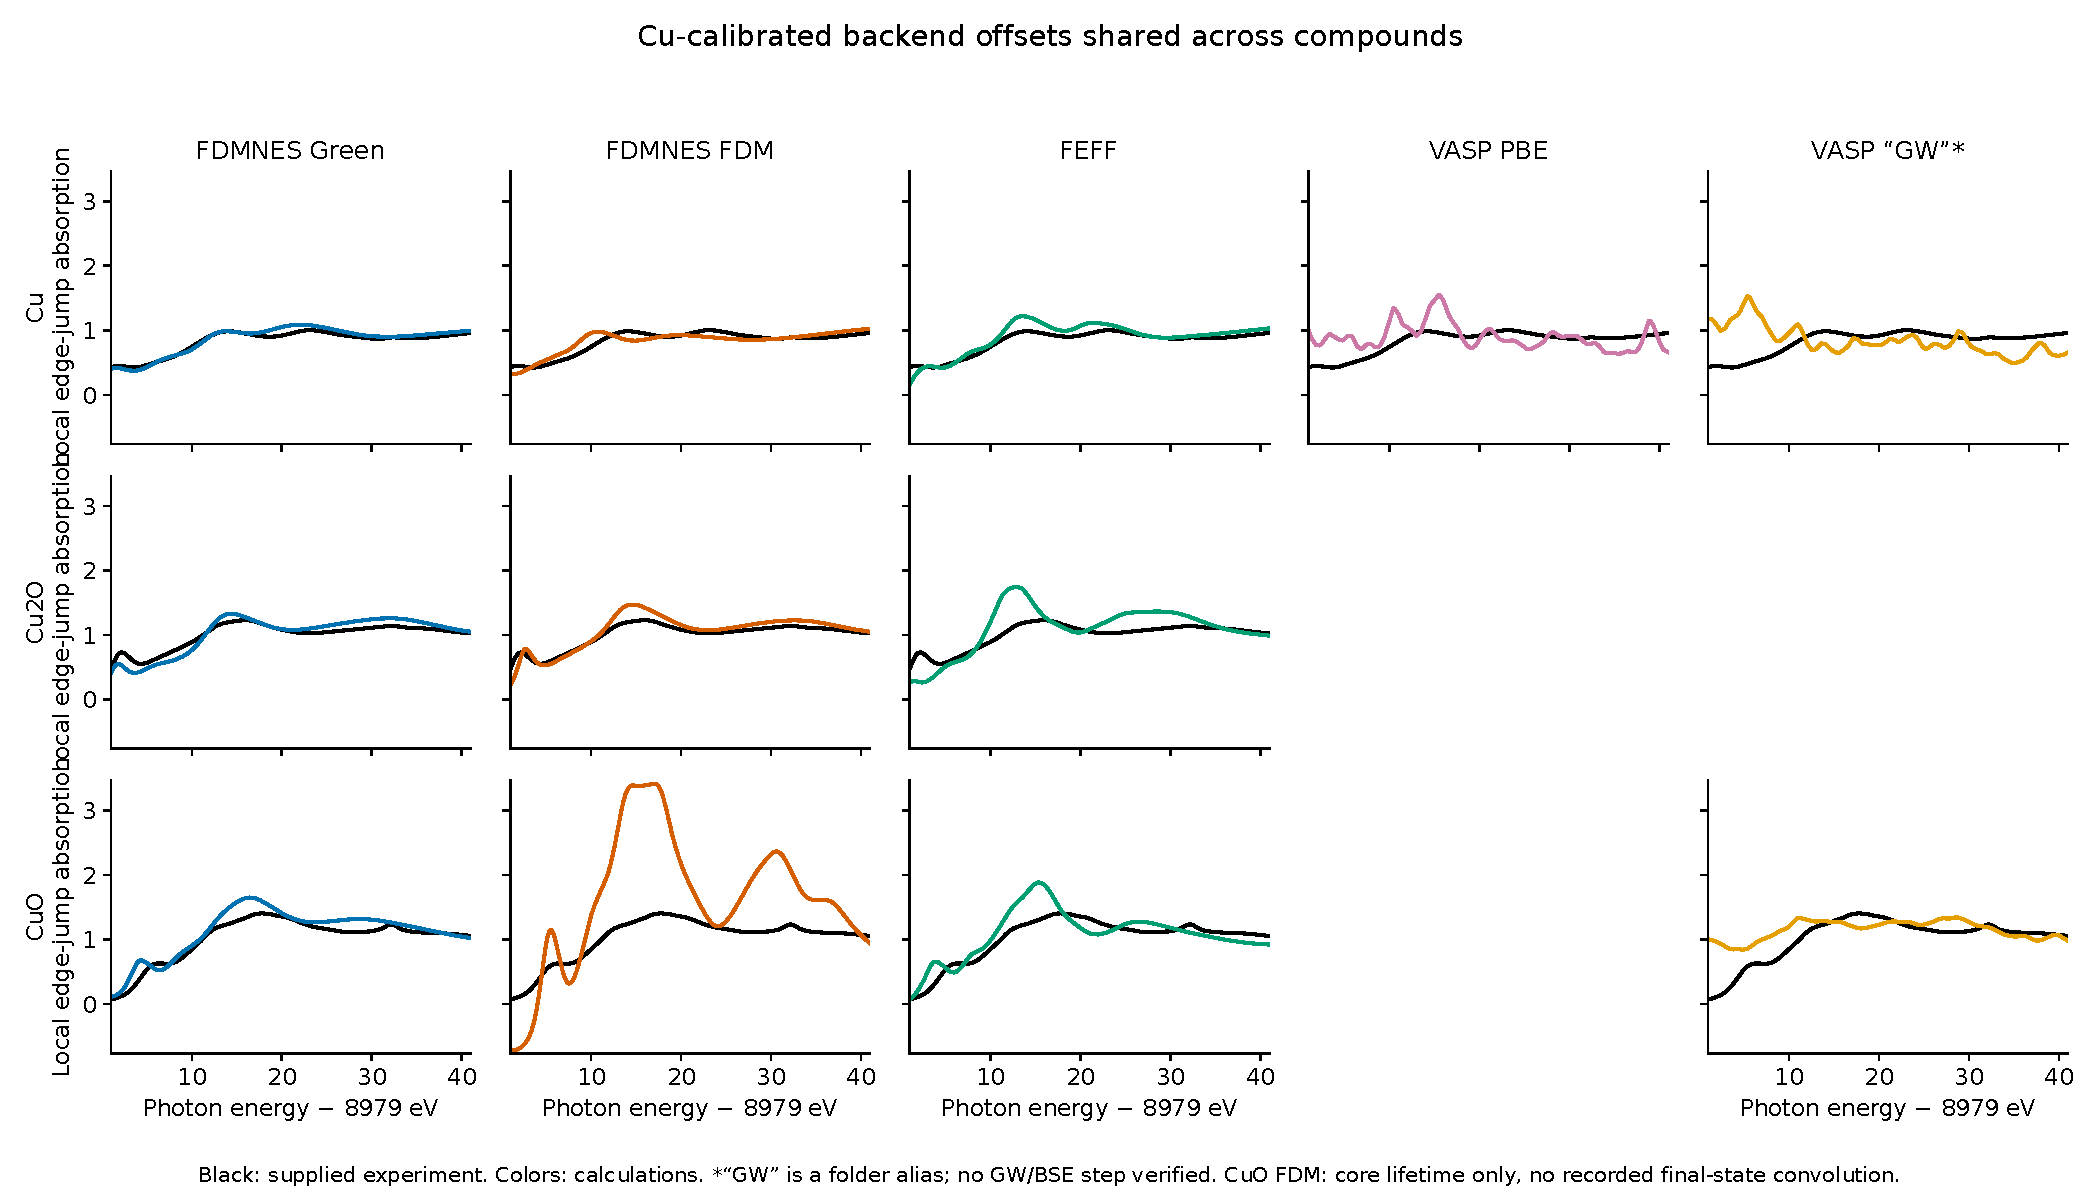
\includegraphics[width=.98\linewidth]{figures/SI_reference_grid_common.pdf}
\caption{Complete three-material, five-computation grid on common Cu-calibrated backend axes. Experiment is black and each method has a consistent color. Blank slots are missing numeric calculations. ``GW'' is an input-directory alias. CuO FDM has no recorded native final-state convolution. All plotted arrays and native inputs are supplied.}
\end{figure}
\end{landscape}
\clearpage
\begin{landscape}
\begin{figure}[p]
\centering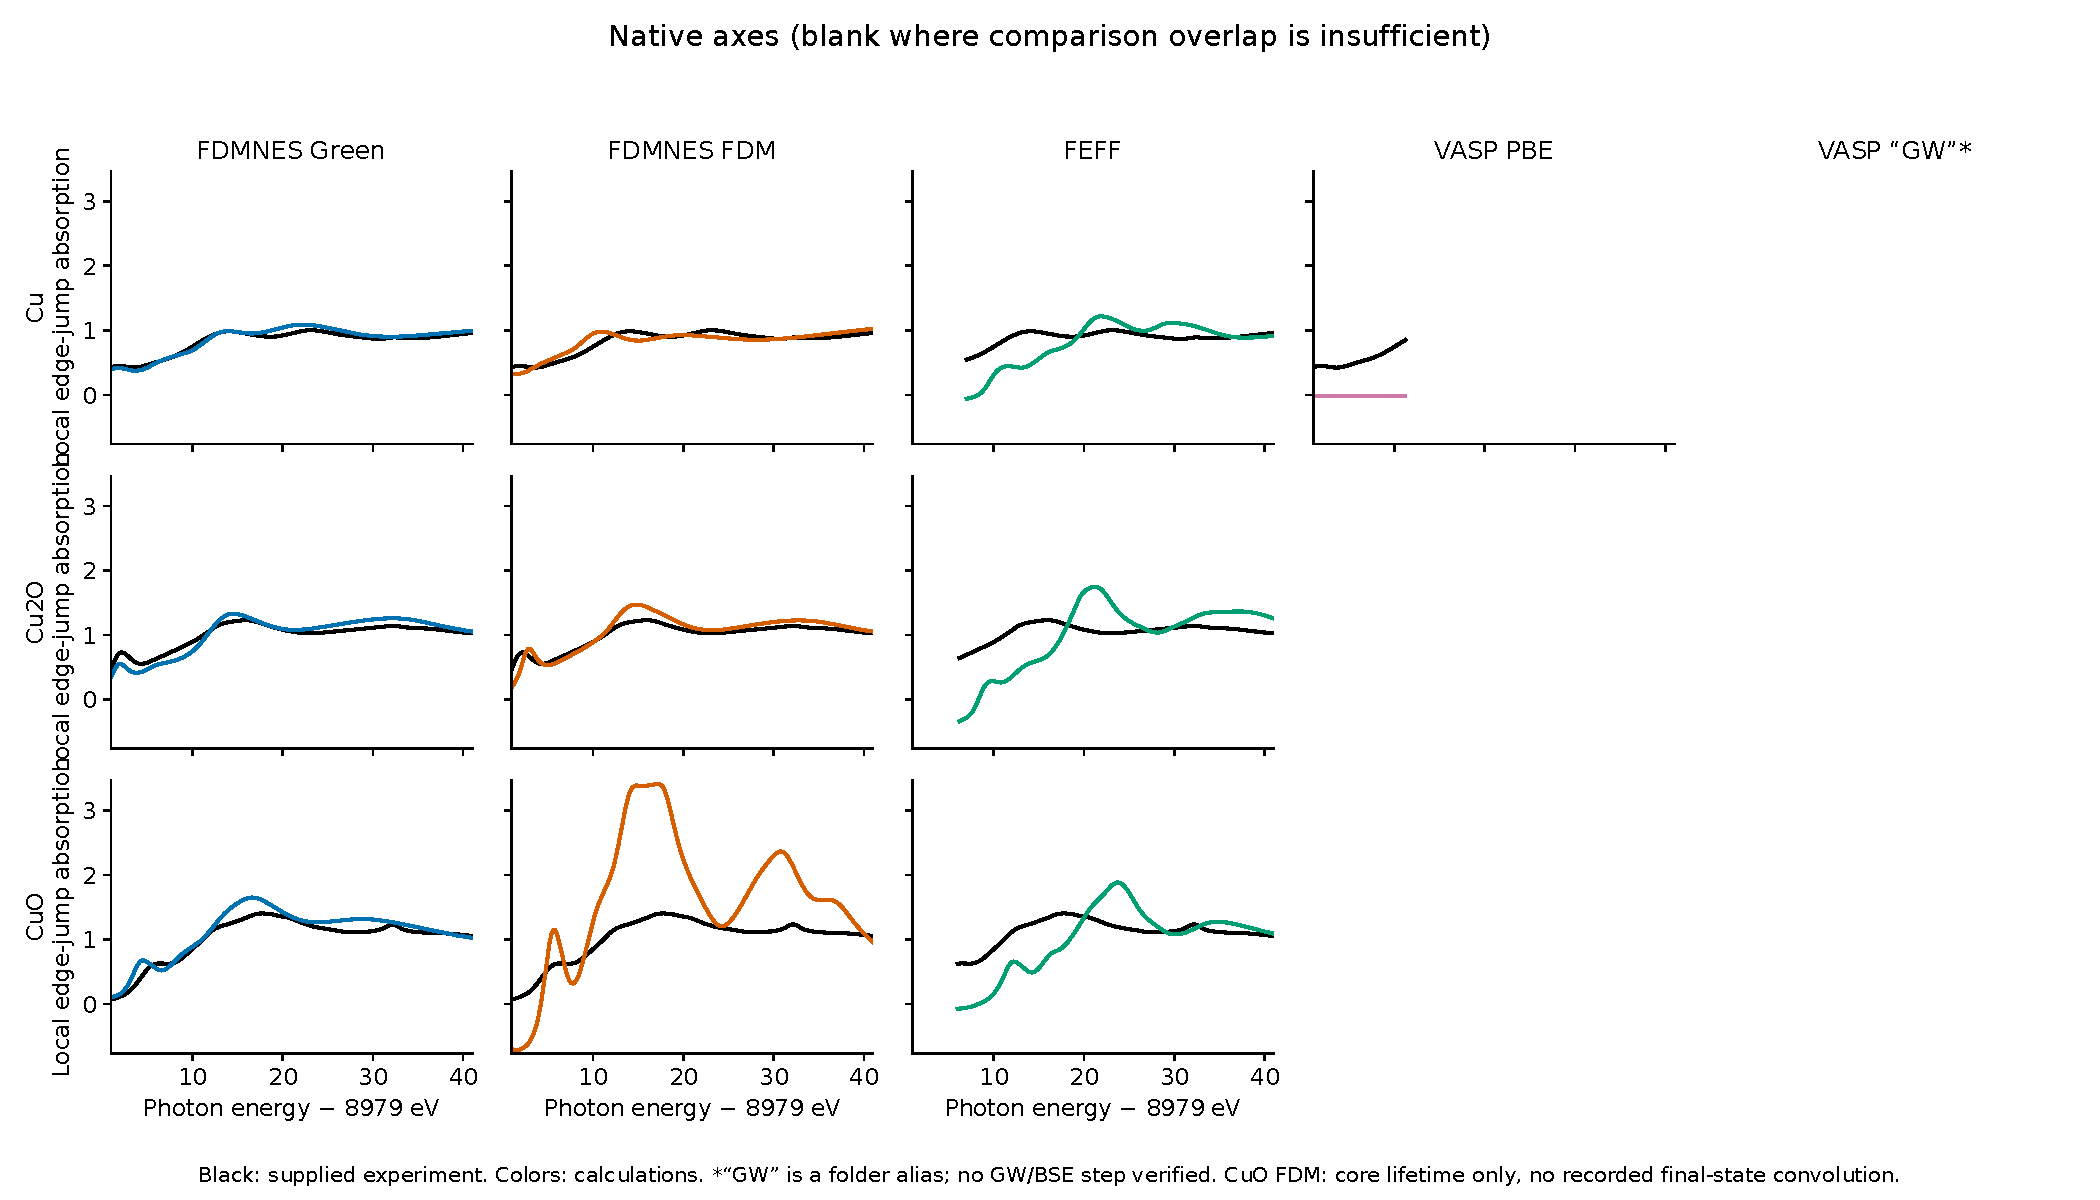
\includegraphics[width=.98\linewidth]{figures/SI_reference_grid_native.pdf}
\caption{Native input axes with zero fitted shift. Only supported intersections are compared. Blank cells also include insufficient overlap. VASP core-excitation axes lack absolute photon calibration; a small tail-only overlap is not evidence of an accurate edge.}
\end{figure}
\end{landscape}
\clearpage
\begin{landscape}
\begin{figure}[p]
\centering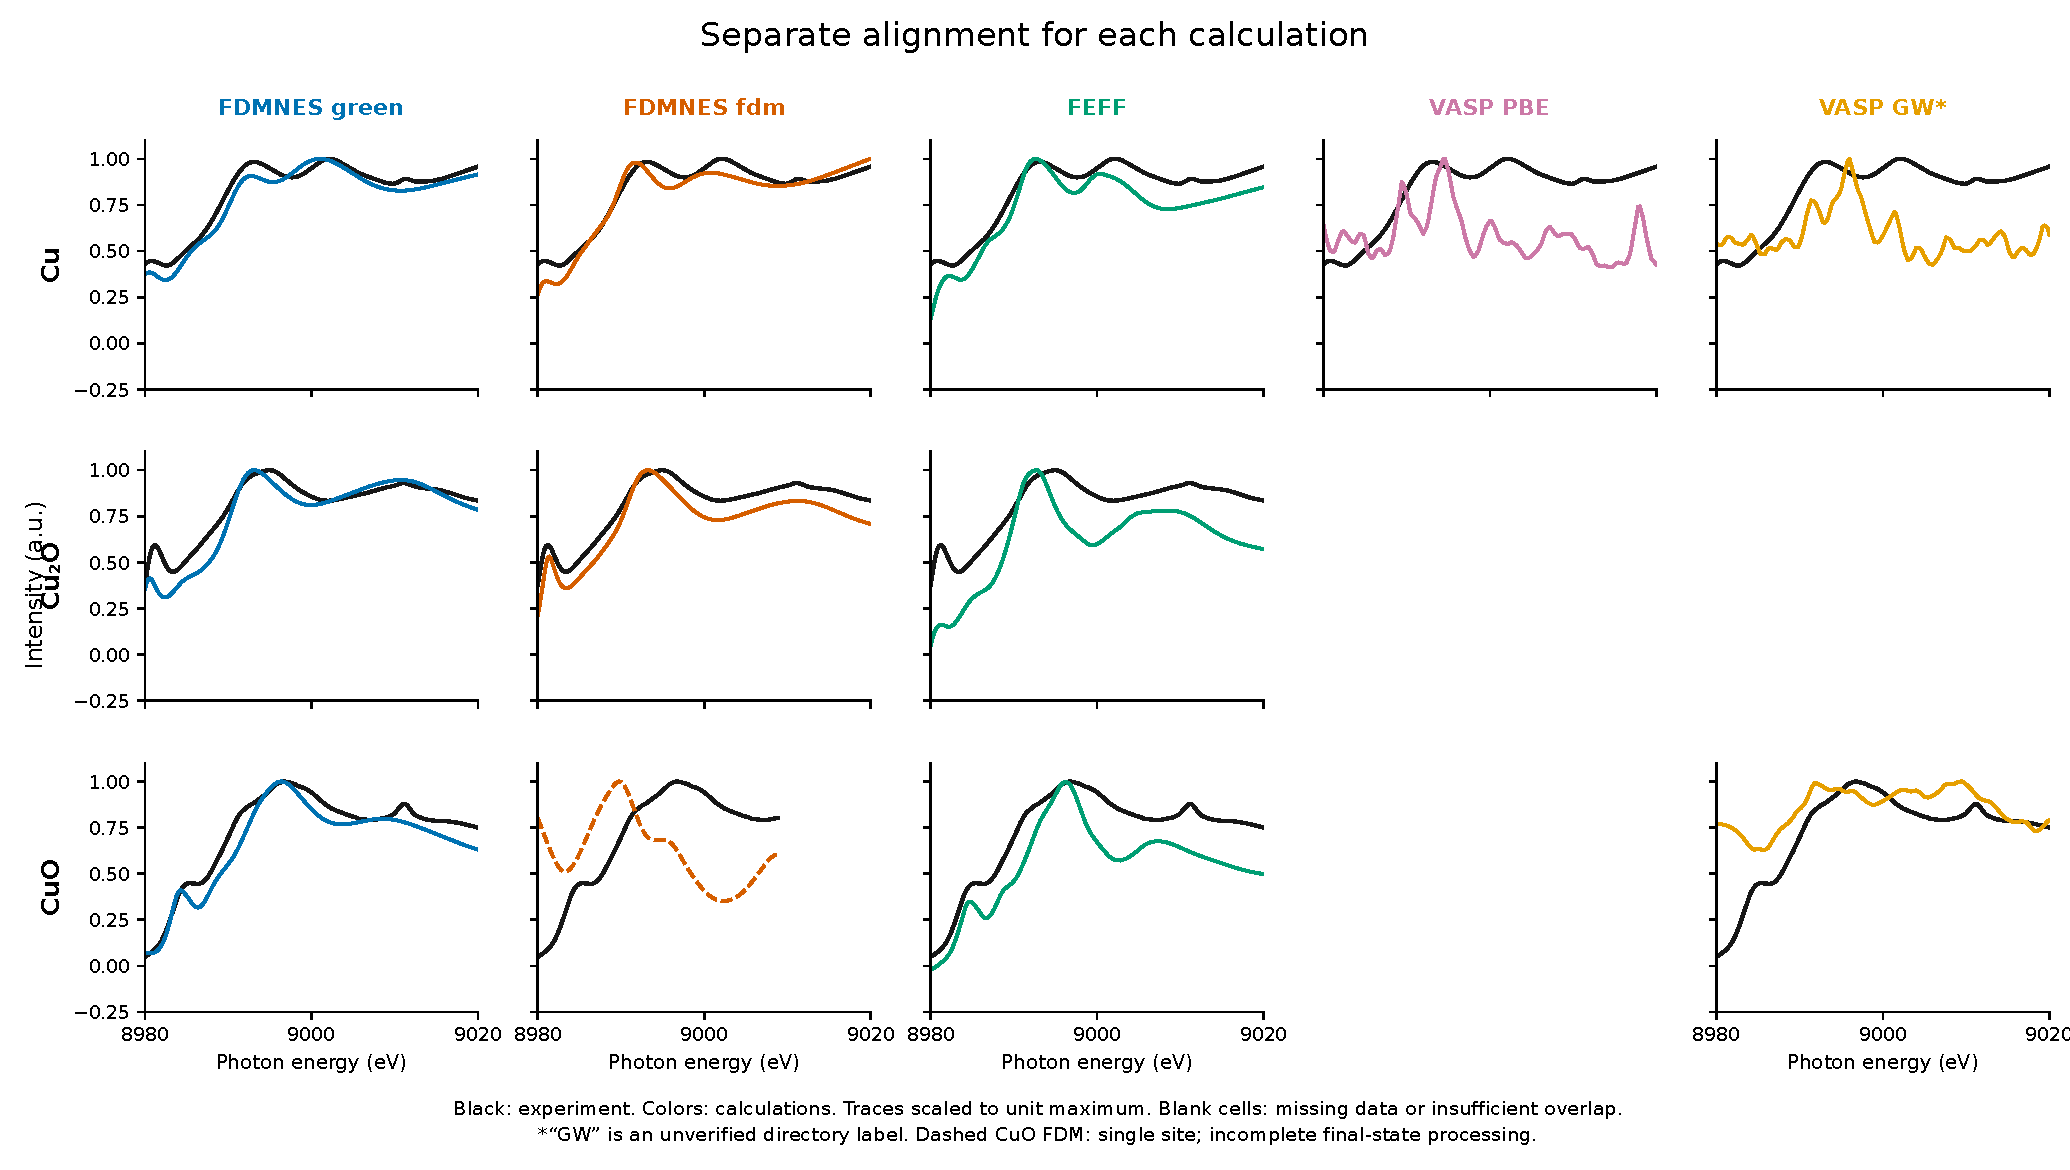
\includegraphics[width=.98\linewidth]{figures/SI_reference_grid_shape_aligned.pdf}
\caption{Separately fitted shape alignment, one bounded residual shift per available compound/method. This view removes chemical shifts and is distinct from the common-offset and native-axis views.}
\end{figure}
\end{landscape}
\clearpage
\begin{landscape}
\begin{figure}[p]
\centering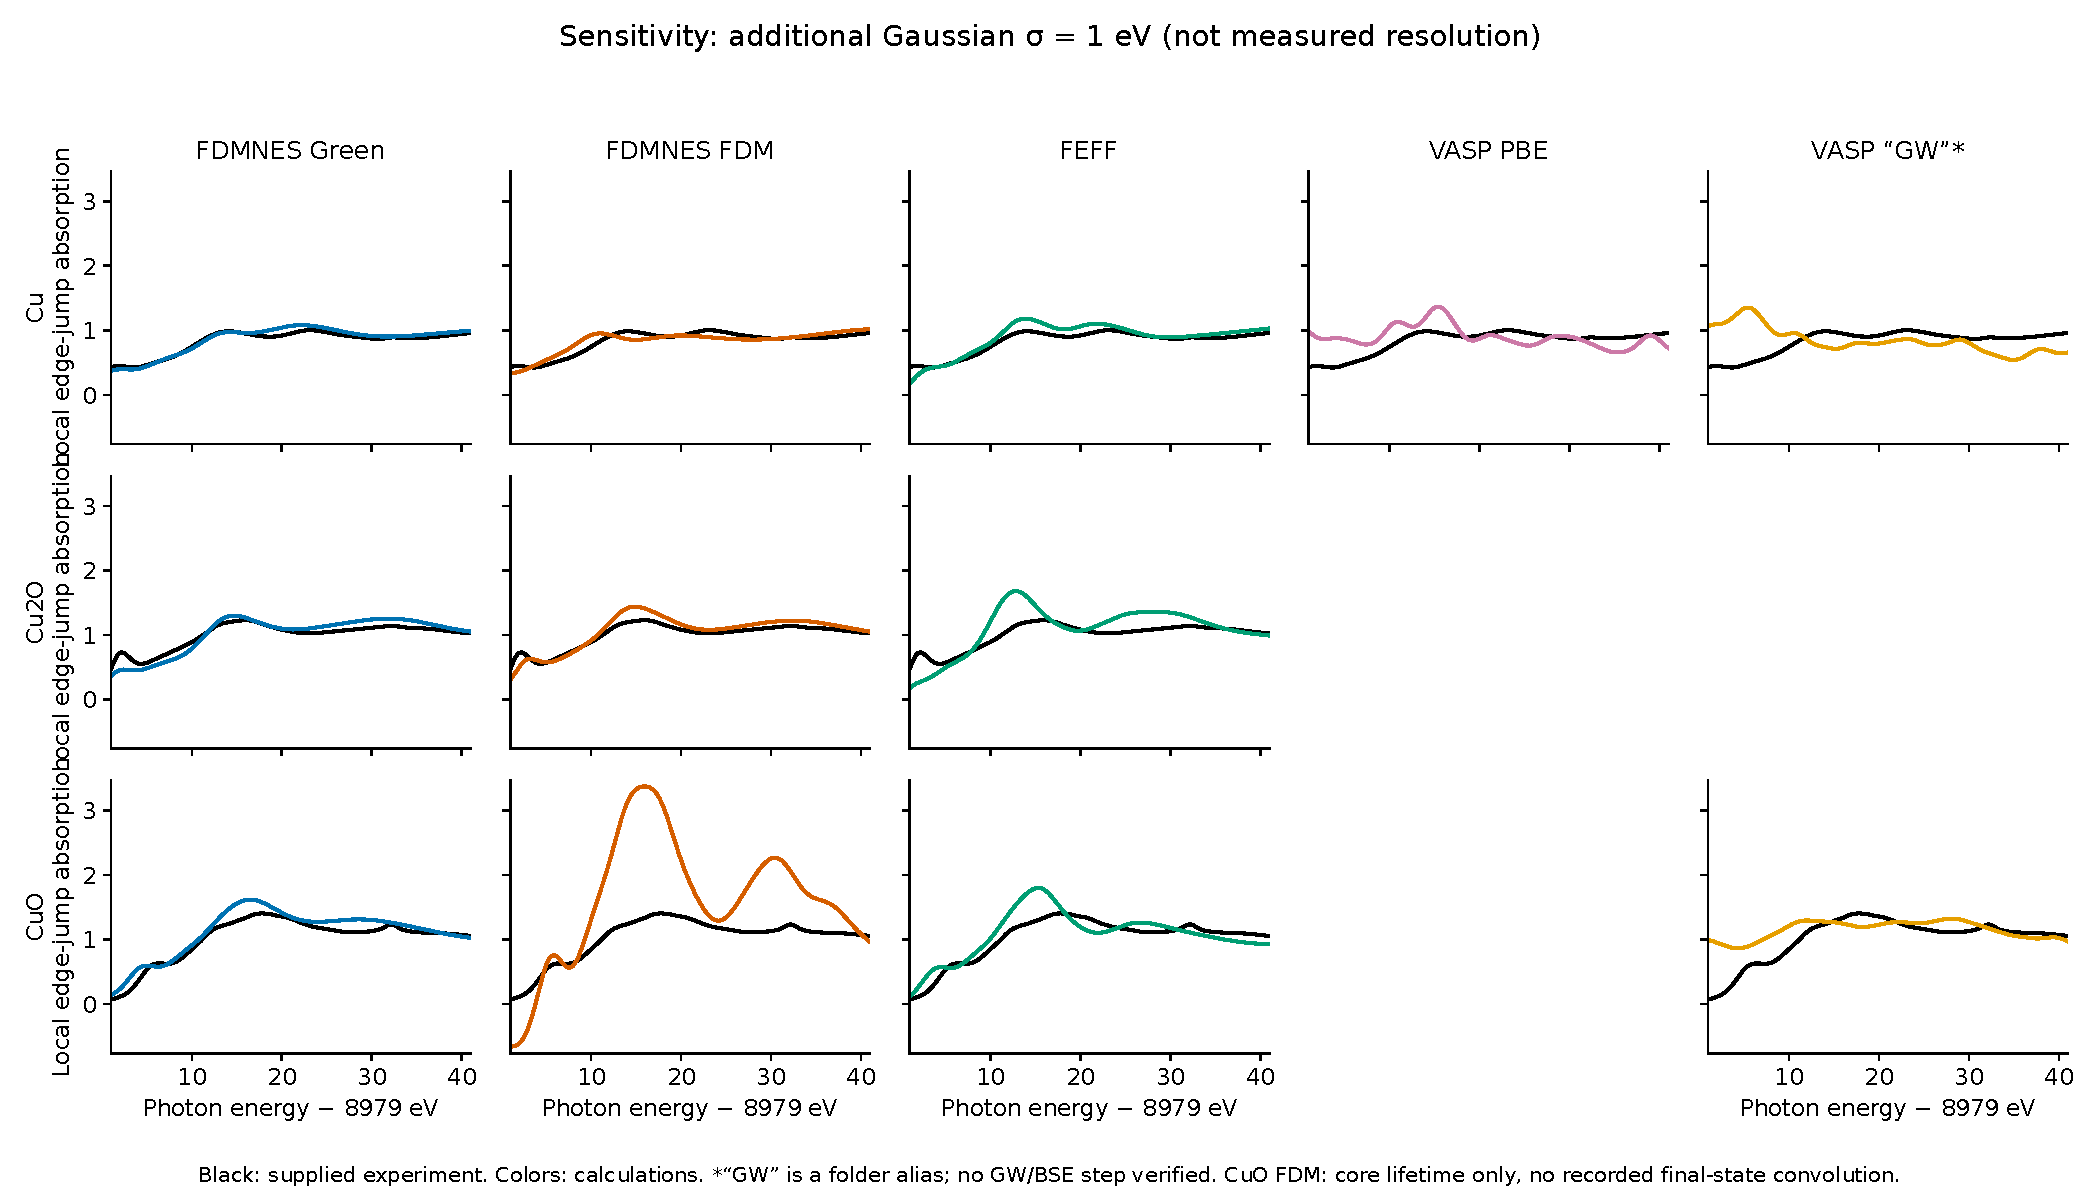
\includegraphics[width=.98\linewidth]{figures/SI_reference_grid_sigma1_sensitivity.pdf}
\caption{Sensitivity to the original notebook's additional Gaussian $\sigma=1$~eV (FWHM 2.35482~eV), at the common offsets. This width is an unvalidated sensitivity parameter, not a measured instrumental resolution. Primary native convolutions are preserved.}
\end{figure}
\end{landscape}
\clearpage


\begin{thebibliography}{99}
\bibitem{vasp1996} G. Kresse and J. Furthm\"uller, Efficient iterative schemes for ab initio total-energy calculations using a plane-wave basis set, \textit{Phys. Rev. B}, 1996, \textbf{54}, 11169--11186, DOI: \href{https://doi.org/10.1103/PhysRevB.54.11169}{10.1103/PhysRevB.54.11169}.
\bibitem{joly2001} Y. Joly, X-ray absorption near-edge structure calculations beyond the muffin-tin approximation, \textit{Phys. Rev. B}, 2001, \textbf{63}, 125120, DOI: \href{https://doi.org/10.1103/PhysRevB.63.125120}{10.1103/PhysRevB.63.125120}.
\bibitem{fdmnesmanual} Y. Joly, \textit{FDMNES User's Guide}, November 2022, \url{https://data-analysis.synchrotron-soleil.fr/tmp/software/fdmnes/fdmnes_Linux/Doc/Manual_Eng.pdf}, accessed 21 October 2026.
\bibitem{rehr2010} J. J. Rehr, J. J. Kas, F. D. Vila, M. P. Prange and K. Jorissen, Parameter-free calculations of X-ray spectra with FEFF9, \textit{Phys. Chem. Chem. Phys.}, 2010, \textbf{12}, 5503--5513, DOI: \href{https://doi.org/10.1039/B926434E}{10.1039/B926434E}.
\bibitem{vaspxas} VASP Wiki, Supercell core-hole calculations, \url{https://vasp.at/wiki/index.php/SCH_calculations}, accessed 21 October 2026.
\bibitem{ahmed1974} N. Ahmed, T. Natarajan and K. R. Rao, Discrete cosine transform, \textit{IEEE Trans. Comput.}, 1974, \textbf{C-23}, 90--93, DOI: \href{https://doi.org/10.1109/T-C.1974.223784}{10.1109/T-C.1974.223784}.
\bibitem{geurts2006} P. Geurts, D. Ernst and L. Wehenkel, Extremely randomized trees, \textit{Mach. Learn.}, 2006, \textbf{63}, 3--42, DOI: \href{https://doi.org/10.1007/s10994-006-6226-1}{10.1007/s10994-006-6226-1}.
\end{thebibliography}

\end{document}
